\lstset{language=PHP}

\section{\mt{Api szerver}{Api server}}

\block{
	\subsection{\mt{Felépítés}{}}
	
	\subsubsection{\mt{Átirányítási réteg}{}}
	
	\p{\mt{%
		A \code{.htaccess} -nek köszönhetően minden beérkező kérés az \code{index.php} fájlba érkezik, amely ezt követően a \code{src/Routing/Router.php} fájlba továbbítja azokat. 
		A Router.php fájl megvizsgálja a kérések URL -jét és metódusát, majd a query kivételével dekódolja és továbbítja az URL paramétereket a \code{src/API} mappában található fájlokba.
	}{}}
}

\block{
	\subsubsection{\mt{API kezelő réteg}{}}
	
	\p{\mt{%
		Az API kérések értelmezése és az engedélyek ellenörzése, illetve az azokra való válasz küldése a \code{src/API} mappában lévő fájlok feladata.
		A kérések formátumának ellenörzéséért például a \code{src/API/APIUtils.php} fájl felelős.
	}{}}
}

\block{
	\subsubsection{\mt{Adatbázis kapcsolat réteg}{}}
	
	\p{\mt{%
		A \code{src/Database} mappában található fájlok feladata az adatbázissal való kapcsolat megteremtése és az adatbázis műveletek kezelése.
	}{}}
}

\block{
	\subsection{ApiRouter.php}
	
	\p{\mt{%
			Amennyiben a kérés metódusa megegyezik a \code{\$method} -al, illetve a kérés URL -je hasonlít a \code{\$pattern} -ben található mintával, a route funkció feladata, hogy lefuttassa a code{\$function} funkciót az URL -ből kiszedett és dekódolt paraméterekkel.
		}{}
		
		\lstinputlisting{generated/api.routing.route.php}
	}
}

\p{\mt{%
		Az API -ra érkező kérés hatására a \code{handle} nevű funkció hívódik meg, amely a \code{route} segítségével átirányítja a dekódolt kéréseket az api kezelő rétegbe.
	}{}
	
	\lstinputlisting{generated/api.routing.handle.php}
}

\block{
	\subsection{APIUtils.php}
	
	\p{\mt{%
			A validate funkció feladata megvizsgálni, hogy a \code{\$data} értéke a \code{\$template} szerint van-e formázva.
			Amennyiben a  \code{\$template} egy szöveg, akkor a funkció a \code{\$data} típusát ellenőrzi.
			Ilyen értékek például:
		}{}

		\begin{itemize}
			\item "string"
			\item "integer"
			\item "double"
		\end{itemize}

		(Ha a \code{\$template} szerint tört szám kell, akkoraz egész szám is elfogadott, mivel egyszerűen átalakítható.)
	}
}

\p{\mt{%
		Amennyiben a \code{\$template} egy lista, ellenőrzi, hogy a \code{\$data} is lista-e.
		Ezt követően a \code{\$template} az első elemét használja mintaként és rekurzívan ellenőrzi a \code{\$data} lista elemeit.
		Ilyen értékek például:
	}{}

	\begin{description}
		\item[["string"]] \mt{Olyan listákat fogad el amiben csak szövegek vannak.}{}
		\item[["integer"]] \mt{Olyan listákat fogad el amiben csak egészek vannak.}{}
		\item[[["double"]]] \mt{Olyan listákat fogad el amiben csak törtszám listák vannak.}{}
	\end{description}
}

\p{\mt{%
		Abban az esetben, ha a \code{\$template} egy asszociatív lista, a validate funkció ellenőrzi, hogy a \code{\$data} is asszociatív lista e.
		Ezt követően a \code{\$template}, saját értékeit mintaként használva, rekurzívanellenőrzi a \code{\$data} értékeit.
		Amennyiben a \code{\$template} kulcsa "?" -el végződik, nincs szükség rá, hogy a \code{\$data} -nak is meglegyen.
		Ilyen értékek például:
	}{}

	\begin{description}
		\item[["key"=>"integer"]] \mt{Ez elfogadja a \code{["key"=>10]} értéket.}{}
		\item[["key?"=>"string"]] \mt{Ez elfogadja a \code{["key"=>"szöveg"]} és \code{[]} értékeket.}{}
	\end{description}
}

\p{
	\lstinputlisting{generated/api.apiutils.validate.php}
}

\begin{landscape}
	\begin{figure}
		\centering
		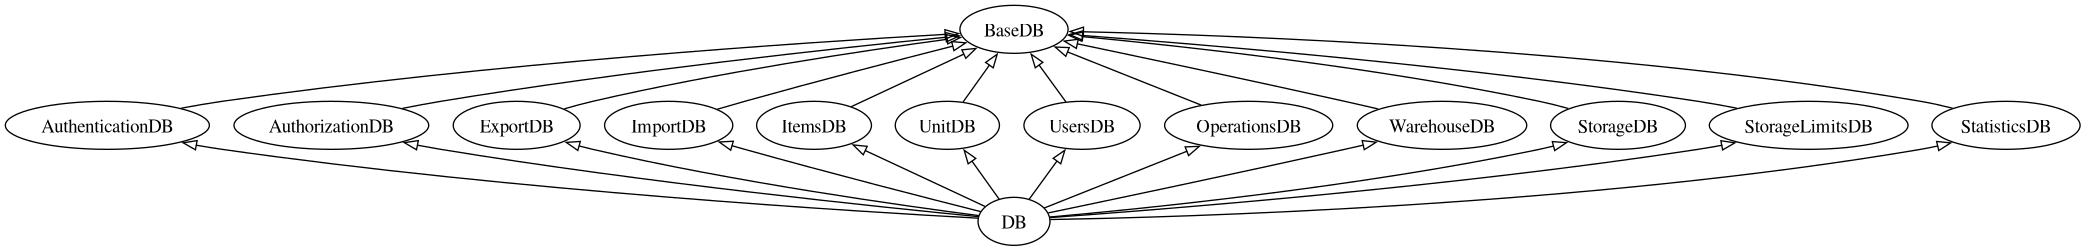
\includegraphics[width=\linewidth]{apiserver.classes.png}
		\caption{\mt{Osztálydiagramm}{}}
	\end{figure}
\end{landscape}

\block{
	\subsection{\mt{DB.php}{}}
	
	\p{\mt{%
		A \code{DB} osztály felelős az adatbázishoz való kapcsolódásért.
		A legtöbb metódus külön \code{trait}-ekben van implementálva, melyeket ez az osztály használ.
		Ez a megoldás nagyban javítja az olvashatóságat, mivel a hasonló feladatokat ellátó funkciók ugyanabban a fájlban vannak és nem mind a \code{DB.php}-ban.
	}{}}
}

\block{
	\subsection{\mt{BaseTrait.php}{}}
	
	\p{\mt{%
		Sok hasznos SQL lekérdezéssel foglalkozó metódus van implementálva a \code{BaseTrait}-ben, így az összes többi \code{trait} használja a \code{BaseTrait}-et ezeknek a bizonyos funkcióknak az eléréséhez.
	}{}}
}

\block{
	\subsection{\mt{Logger.php}{}}
	
	\p{\mt{%
			A \code{Logger} osztály az eseménynapló kezelésével foglalkozik.
		}{}
		
		\lstinputlisting{generated/api.logger.php}
	}
}

\block{
	\subsection{\mt{Settings.php}{}}
	
	\p{\mt{%
			A \code{Settings} osztály a \code{config.json} olvasásáért felelős.
		}{}
		
		\lstinputlisting{generated/api.settings.php}
	}
}

\block{
	\subsection{\mt{Authentication.php}{}}
	
	\p{\mt{%
			A \code{Authentication} osztály a hiteletísért felelős.
		}{}
		
		\lstinputlisting{generated/api.authentication.php}
	}
}

